\begin{figure}[htb!]
    \centering
    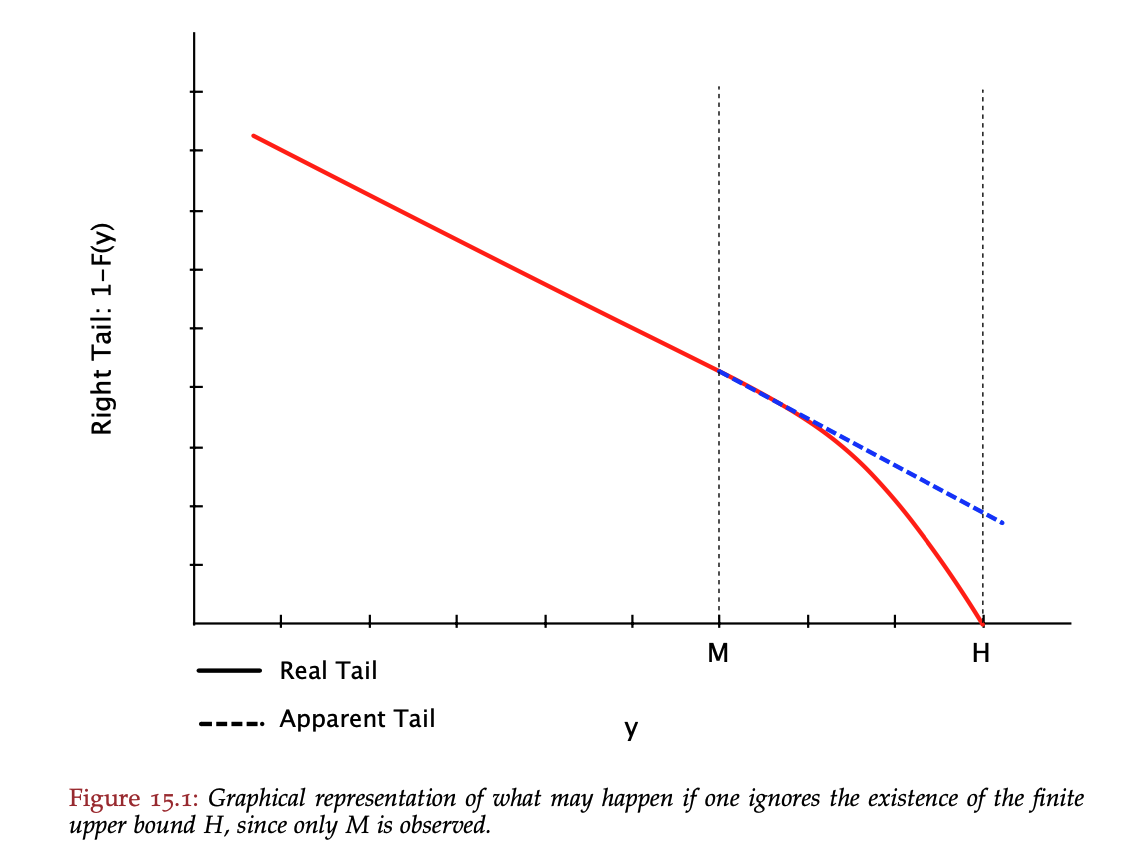
\includegraphics[width=1\linewidth]{images/nnt-upper-bound.png}
    \vspace{-15pt}
   \caption{As shown in this Figure from T19~\cite{taleb2019statistical} if you only
   observe a distribution up to some value M, you may be tempted to fit a line through the
   data (dotted blue line). But if there were in fact a limit to the distribution at H,
   you would be overestimating the true number of very extreme events (red curve) and also predict
   events that were larger than were possible.  }
   \label{fig:up-bound-taleb}
   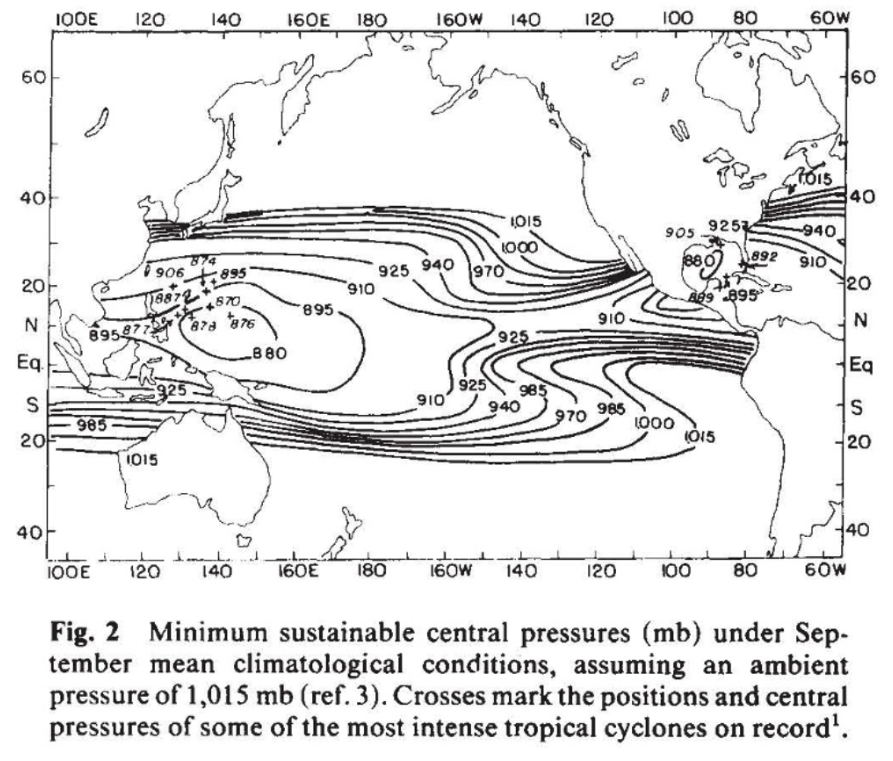
\includegraphics[width=1\linewidth]{images/hurricane-Emanuel-upper-bound.png}
   \vspace{-15pt}
  \caption{From Emanuel, Nature (1987)~\cite{emanuel1987dependence}
  (Automatically Updated Version: \url{http://wxmaps.org/pix/hurpot}).
  The data on the graph shows that at the time the minimum central pressure
  closely matched the limits predicted in~\cite{emanuel1986air}. }
   \label{fig:emanuel87}

\end{figure}

A shown in Figure~\ref{fig:up-bound-taleb}
